\documentclass[12pt,UTF8,a4]{article}
\usepackage{amsmath}
\usepackage{indentfirst}
\usepackage{multirow}
\usepackage{titlesec}
\usepackage{graphicx}
\usepackage{longtable}
\usepackage{framed}
\usepackage[noend]{algorithmic}
\usepackage{algorithm}
\usepackage{sectsty}
\usepackage{setspace}
\usepackage[footnotesize]{caption}
\usepackage{enumitem}
\usepackage[text={18cm,24cm}]{geometry}
\usepackage[hyperfigures,bookmarksnumbered,bookmarksopen,bookmarks,colorlinks,citecolor=blue,linkcolor=blue]{hyperref}
\usepackage{natbib}

\setlength{\bibsep}{0.0pt}
\algsetup{indent=2em}
\setlength{\parindent}{2em} \setlength{\parskip}{3pt plus1pt minus1pt}

\sectionfont{\large}
\subsectionfont{\normalsize}
\paragraphfont{\small}

\singlespacing
\title{CSCE 604 Final Project Report \\ Design and Implementation of a 2D Programming Language}
\author{Robert Schumacher, Plamen Ivanov and Peihong Guo}
\date{\today}

\begin{document}
\maketitle
\singlespacing

\section{Introduction}
We designed and implemented a two dimensional programming language featuring an interactive graphical programming environment in this project.

\section{Design Decisions}
\subsection{Basic Framework}
A program in the 2D programming language is a collection of definitions. A definition is the basic building block, which may contain predefined definitions, special definitions and user defined definitions.

Predefined definitions include \texttt{print}, \texttt{pair}, \texttt{first} and \texttt{second}.

Special definitions include \texttt{input}, \texttt{output}, \texttt{if}, \texttt{constant} and \texttt{arithmetic}.

The system maintains a global list of definitions, including predefined ones and special ones. These definitions are referenced wherever needed, such as inside the body of a specific definition. 

\subsubsection{Structure of Definition}
Each definition consists of input, output, and a definition body. The body of a definition may include other definitions, such as predefined definitions or user-defined definitions.

The input of a definition can be empty, which corresponds to a definition that does not require an input. Definitions of this type are \texttt{input}, \texttt{constant}.

The body of a definition is a set of nodes referring to definitions. The member nodes of a definition are connected by a set of edges indicating the input-output dependencies between nodes, as is shown in Figure.~\ref{fig:defbody}.

\begin{figure}[h]
\center
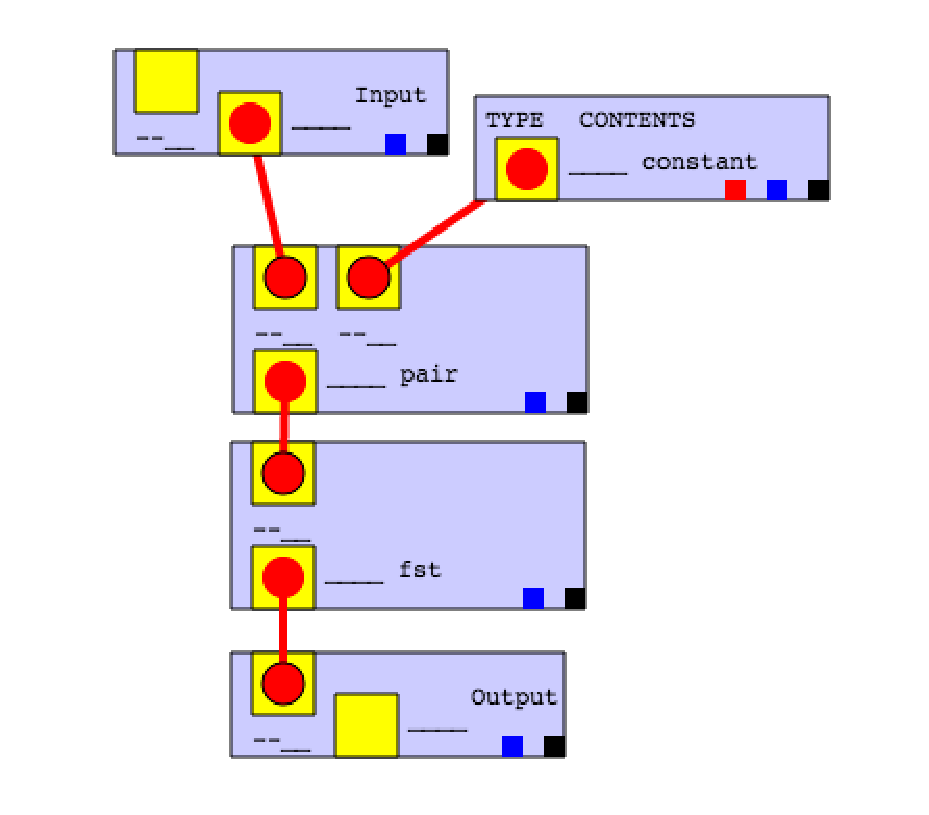
\includegraphics[width=0.75\textwidth]{./images/defbody.eps}
\end{figure}

\subsection{Graphical Interface}


\subsection{Language Design}
\section{Implementation Details}
\subsection{GUI}
\subsection{Type-checking and Evaluation}
\section{Conclusion}

\end{document}
